\subsection{Designing Simple Change} % (fold)
\label{sub:designing_simple_change}

Table \ref{tbl:storing-data-prog} contains a description of the next program we are going to design. This program will calculate and output the ideal change for a given transaction from a Vending Machine. In designing this program we will make use of the concepts introduced in this chapter; we will use a Function to calculate the coins to give, Variables to store values such as the amount paid, Constants for the values of the different coins, and Parameters to pass values to the Function.

\begin{table}[h]
\centering
\begin{tabular}{l|p{10cm}}
  \hline
  \multicolumn{2}{c}{\textbf{Program Description}} \\
  \hline
  \textbf{Name} & \emph{Simple Change Calculator} \\
  \\
  \textbf{Description} & Calculates the idea change for a given transaction in a Vending Machine. The transaction involves reading the cost of the item purchased and the amount paid, and then outputting the number of each type of coin to give as change.\\
  \hline
\end{tabular}
\caption{Description of the Simple Change Calculator program.}
\label{tbl:storing-data-prog}
\end{table}


To design and implement this program we need to follow a number of steps:
\begin{enumerate}
  \item Understand the problem, and get some ideas on the tasks that need to be performed.
  \item Choose the artefacts we will create and use
  \item Map these artefacts to code
  \item Compile and run the program
\end{enumerate}

In step 1 you need to understand what it is that you want the program to do. This will involve determining the tasks to be performed, the steps involved in those tasks, and any data associated with them. Once you have a good understanding of what you want to achieve you can start to build a solution. In this step you determine the artefacts you want to create, and try to locate those you could use from the available libraries. Step 3 then turns your plans into source code that can be compiled and run in Step 4. 

% subsection designing_simple_change (end)

\subsection{Understanding the Simple Change Calculator} % (fold)
\label{sub:understanding_simple_change}

Receiving change from a transaction is something that you should be familiar with, and determining the ideal change is not an overly complex task. While the task itself is common, it does not mean that you can skip thinking about it. If you had to give \$6.50 in change you know without thinking that you should give three \$2 coins, and one 50c coin. What you need to do now is think through the steps that you perform intuitively.

Think about all the steps for how you actually calculated the change to be given. The first \emph{secret} is to realise that you need to start with the coin with the largest value, and then work down from there to the coin with the smallest value. The number of coins you give each time can then be calculated by dividing the amount of change to be given by the value of the current coin. Lastly you need to reduce the amount of change remains to be given. These steps are shown in the pseudocode in Listing \ref{lst:data-simple-change-pseudo}.

\pseudocode{lst:data-simple-change-pseudo}{Pseudocode for Simple Change program.}{./topics/storing-using-data/application/CalculateChange.txt}
% subsection understanding_simple_change (end)

\subsection{Choosing Artefacts for the Simple Change Calculator} % (fold)
\label{sub:choosing_artefacts_for_simple_change}

Designing data is much like designing the procedures in your program. You need to think about the solution and try to identify the different values that are being used. Each of these values can then become either a Variable, a Parameter, or a Constant. Looking over the steps for calculating change you should be able to identify several different kinds of values. You need to be able to store the cost of the item being purchased, the amount of money paid, and the amount of change you need to give. Each of these can then become local variables within the program's main instructions.

Thinking further about the problem you should also be able to identify the constant values needed to model the different coins. These values are almost taken for granted when you think about it yourself, but the computer is unintelligent, so you need to specify everything for it. Using constants is a better option than hard coding these values directly in the program, so each of these value can be coded as a Constant.

Next you need to think about each function or procedure, and determine if it requires data to be given to it to enable it to perform its action. Any data it requires must then be passed to it using Parameters. In the design of this program there is one function and one procedure. The function, \texttt{Coins to Give}, calculates the number of coins of a certain value that must be given in the change. This function must be told the value of the \texttt{change}, as well as the \texttt{coin value}. It can then use these two values to determine how many of these coins should be given in the change. Similarly, the \texttt{Output Change Data} procedure will accept the number of coins given, \texttt{number given}, as well as a textual description of the coin, \texttt{Coin Description}. This procedure will have the side effect of writing these details to the Terminal.

The key to understanding Parameters is to remember that each Procedure and Function is its own isolated domain. It can have its own data, using Local Variables, and has its own instructions. In most cases these instructions will need to be given some starting data, some information upon which to act. You can put yourself in the place of the function, or procedure. For example, what would you need to be told in order to determine the number of coins to give in change for a single coin type. You can not work out the answer without being told the value of the change to be given and the value of the coin you are calculating for. With these two pieces of information you now have enough to determine, for example, how many \$2 coins should be given for \$6.50 in change, and you can respond back with the answer 3. This is exactly what is being coded in the \texttt{Coins to Give} function.

In this respect Procedures are the same. In order to output the change data, the Procedure needs some information. It can not act without this information. If you needed to \emph{output change data}, you need to be told something of the data to output. In this case the Procedure needs to be told the number of coins given, \texttt{number given}, and the description of that coin. With these details the Procedure can then code the steps needed to produce its desired side effect.

One of the main keys to understanding programs, and to creating good designs, is to see how each artefact you create models something from the problem. The Procedures that you create model the processes in the task, performing actions that relate to the task at hand. The Functions model calculations that need to be performed, such as determining how many coins should be given. In the same way the Variables that you create will store values related to the problem. Each variable \textbf{represents} something related to the problem. This \emph{thing} should be reflected in the name given to the variable.

The act of trying to model the problem in software is called \textbf{abstraction}. It is the process of determining the features of the problem that are essential to the solution, and capturing these in a way that models reality but keeps only the details we care about. The ability to create your own model is a skill that you learn with experience, taking a lot of practice to really master.

\clearpage

Listing \ref{lst:data-simple-change-pseudo} shows the pseudocode for the Simple Change program. The following list shows the different artefacts being created, and outlines their purpose.

\begin{itemize}
  \item \textbf{Constants}:
  \begin{itemize}
    \item \texttt{\textbf{TWO\_DOLLARS}} with value 200, represents the value of a \$2 coin
    \item \texttt{\textbf{ONE\_DOLLAR}} with value 100, represents the value of a \$1 coin
    \item \texttt{\textbf{FIFTY\_CENTS}} with value 50, represents the value of a 50c coin
    \item \texttt{\textbf{TWENTY\_CENTS}} with value 20, represents the value of a 20c coin
    \item \texttt{\textbf{TEN\_CENTS}} with value 10, represents the value of a 10c coin
    \item \texttt{\textbf{FIVE\_CENTS}} with value 5, represents the value of a 5c coin
  \end{itemize}
  \item \textbf{Variables}:
  \begin{itemize}
    \item \textbf{\texttt{Cost of Item}}: Stores the value of the item being purchased. This design uses cents as its base to make the calculations easier, avoiding rounding issues involved in using floating point values.
    \item \texttt{\textbf{Payment}}: This is used to store the value of the payment being made. Once again this will be in cents.
    \item \texttt{\textbf{Change Value}}: Keeps track of the current amount of change that has to be given to the user.
    \item \texttt{\textbf{To Give}}: Stores the number of the current coin to give in the change.
  \end{itemize}
  \item \textbf{Function}:
  \begin{itemize}
    \item \texttt{\textbf{Coins to Give}}: Calculates the number of coins to give, returning how many of these coins should be dispensed as part of giving this change. This Function has the following \textbf{Parameters}:
    \begin{itemize}
      \item \texttt{\textbf{Change}}: The value of the change that is to be given.
      \item \texttt{\textbf{Coin Value}}: The value of the coin that is being dispensed.
    \end{itemize}
  \end{itemize}
  \item \textbf{Procedure}:
  \begin{itemize}
    \item \texttt{\textbf{Output Change Data}}: Outputs the coin details to the Terminal, showing the number and description of the change to give. This requires the following \textbf{Parameters}:
    \begin{itemize}
      \item \textbf{\texttt{Number Given}}: The number of coins given.
      \item \textbf{\texttt{Coin Description}}: The description of the coin.
    \end{itemize}
  \end{itemize}
\end{itemize}

In addition to these artefacts the program will make use of some Procedures from the Language's libraries. This will include the following:
\begin{itemize}
  \item \textbf{Output}: You need to use the Language's procedures to write output to the Terminal.
  \item \textbf{Input}: The Language will also provide a means of reading values from the user. In C and Pascal these input procedures need to be passed the Variables that you want the value assigned to. This uses Pass by Reference to enable the input Procedure to store the values read into a Variable for the caller.
\end{itemize}

\csection{
In C the input Procedure to read values from the Terminal is called \csnipet{scanf()}, see \nameref{sub:c_terminal_input}.
}

\passection{
In Pascal the main input Procedure to read values from the Terminal is called \passnipet{ReadLn()}
, see \nameref{sub:pas_terminal_input}.}

\begin{figure}[p]
   \centering
   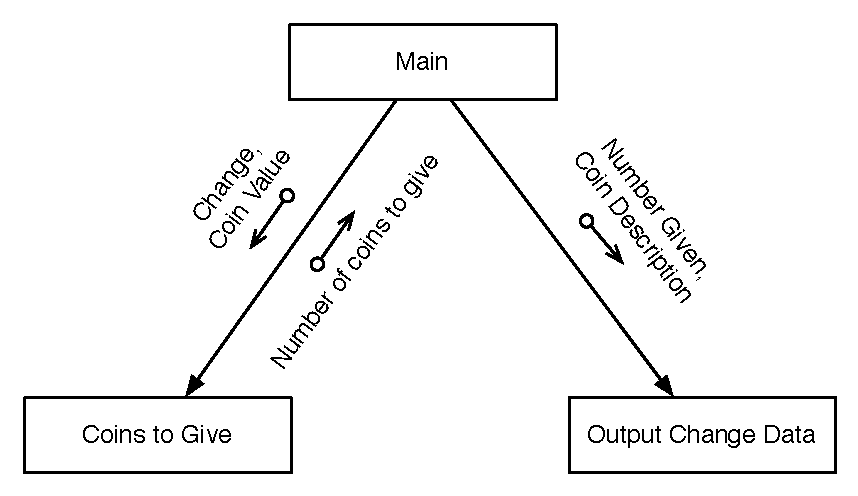
\includegraphics[width=0.7\textwidth]{./topics/storing-using-data/images/SimpleCalcStructure} 
   \caption{Structure Chart for the Simple Change Calculator}
   \label{fig:simple-change-structure}
\end{figure}

\begin{figure}[p]
   \centering
   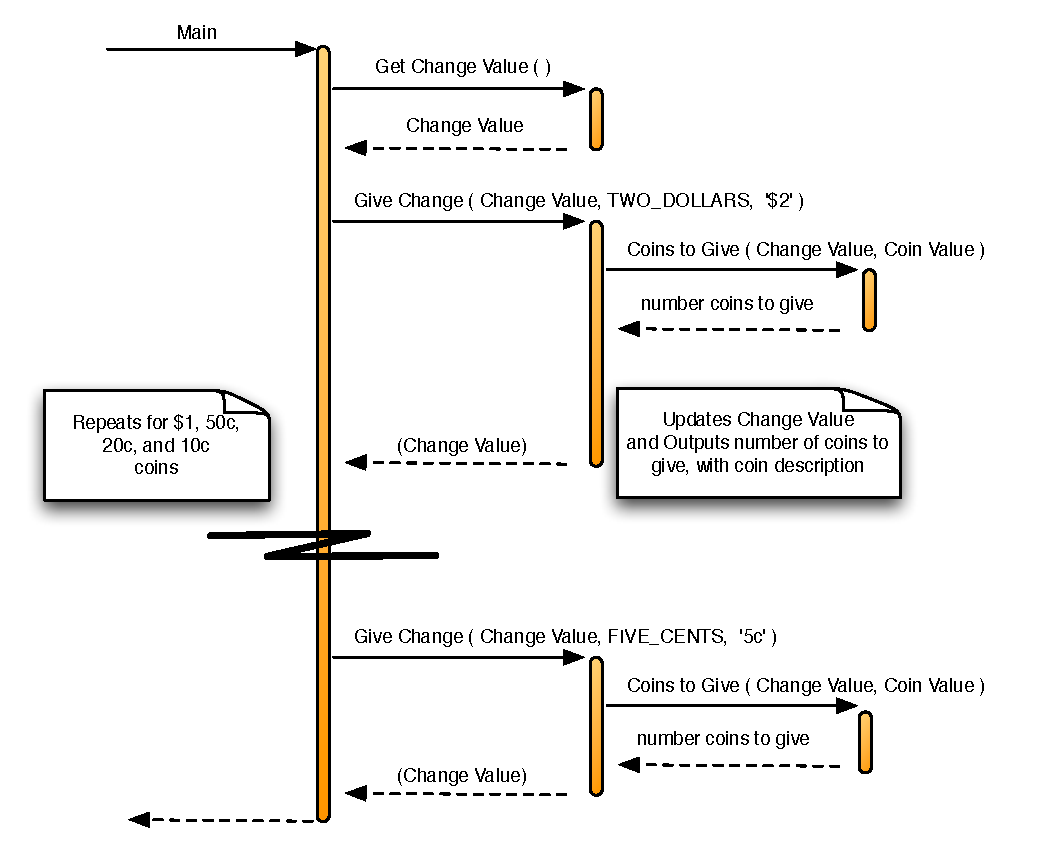
\includegraphics[width=0.8\textwidth]{./topics/storing-using-data/images/SimpleCalcSeq} 
   \caption{Sequence Diagram for the Simple Change Calculator}
   \label{fig:simple-change-seq}
\end{figure}

Figure \ref{fig:simple-change-structure} shows the Structure Chart for the Simple Change Calculator. This shows the structure of the solution, visually showing the Functions and Procedures and the calls between them. This diagram can now be enhanced to show the parameter values being passed into the Functions and Procedures, and the values being returned from the Functions. These data flows are shown alongside the call arrow, with their own smaller arrow to indicate the direction of the flow. By reading Figure \ref{fig:simple-change-structure} you can tell that \texttt{Coins to Give} is going to be a function as it is returning data to \texttt{Main}. Similarly, you can tell \texttt{Output Change Data} is a Procedure as it does not return a value to \texttt{Main}. You can also see that \texttt{Coins to Give} and \texttt{Output Change Data} both require Parameters to accept the data being passed into them from \texttt{Main}. 

The Structure Chart shows the static structure of the code, indicating the calls between the Functions and Procedures, but not communicating when these are called, or how many times. This, more dynamic, information is captured in the Sequence Diagram shown in Figure \ref{fig:simple-change-seq}. This diagram shows the sequence in which the Function and Procedure calls are performed. Notice that this diagram has also been enhanced to show the data that flows into the Functions and Procedures when they are called, as well as the data that is being returned from Functions.

% subsection choosing_artefacts_for_simple_change (end)

\subsection{Writing the Code for the Simple Change Calculator} % (fold)
\label{sub:writing_the_code_for_simple_change}

The pseudocode from Listing \ref{lst:data-simple-change-pseudo} shows the instructions, and how these should be divided between the \texttt{Coins to Give} Function and \texttt{Output Change Data} Procedure. At this stage these instructions need to be translated into source code, so that they can be compiled and the resulting program tested.

The following two sections, Section \ref{sec:storing_and_using_data_in_c} \nameref{sec:storing_and_using_data_in_c} and Section \ref{sec:storing_and_using_data_in_pascal} \nameref{sec:storing_and_using_data_in_pascal}, contain a description of the syntax needed to create programs in the C and Pascal programming languages that include Variable and Function declarations.

\mynote{
Remember the basic process for reading the Syntax Diagrams is to:
\begin{enumerate}
  \item Find the page with the Syntax rule you are interested in knowing about.
  \item Have a quick look at the Syntax Diagram and the rules it contains. Read each rule, and get a basic feel for how it is going to come together for your program.
  \item Read the example to see one way of using the Rule. The Syntax Diagram can be used to create any number of variations of the rule, the example gives you at least one way these rules can be coded.
  \item Return to the diagram and make sure you can match each part of the example back to the rule that created it.
  \item Look up any related rules that are not explained on this rule's page.
\end{enumerate}
}


% subsection writing_the_code_for_simple_change (end)
\clearpage
\subsection{Compiling and Running the Simple Change Calculator} % (fold)
\label{sub:compiling_and_running_simple_change}

Once you have completed your program, you need to compile and test it. 

\begin{enumerate}
  \item Open the \textbf{Terminal}\footnote{The \textbf{MinGW Shell} on Windows.} program for your Operating System
  \item Use the \texttt{\textbf{cd}} command to move to the directory with your code, for example \newline \bashsnipet{cd /Users/acain/Documents/Code}
  \item Run the compiler with your program's code. See the language specific details below.
  \item Fix any compiler errors, using the tips from Section \ref{ssub:compiler_errors} \nameref{ssub:compiler_errors}.
  \item Execute the program using \bashsnipet{./SimpleChange} and check the results
\end{enumerate}

\csection{
The C compiler is called \textbf{gcc}. To compile your \emph{Simple Change Calculator} program you will need to run the following: \newline \newline \bashsnipet{gcc -o SimpleChange simple-change.c}
}

\passection{
The Pascal compiler is called \textbf{fpc}. To compile your \emph{Simple Change Calculator} program you will need to run the following: \newline \newline \bashsnipet{fpc -S2 SimpleChange.pas}
}

\subsubsection{Generating Test Data} % (fold)
\label{ssub:generating_test_data}

Now that our program is making greater use of data it becomes more important to think about how to test your program. Testing is the process of trying to locate issues with your code. There are two main classifications for issues, \textbf{syntactic errors} and \textbf{semantic errors}.

Syntactic errors indicate places in your code where you have not correctly followed the syntax of the language. These are the easiest kind of error to find as the compiler will not be able to compile the program if its syntax is not correct. The errors that the compiler report are all syntax errors. As you gain experience with a Language you will find that you make fewer and fewer of these kinds of errors. 

Semantic errors, on the other hand, will not be found by the compiler. These are errors in the logic within the program. They are cases where you have correctly structured the code, but the code itself does not get the computer to perform the actions you require. These are the kinds of errors that you need to learn to be able to detect yourself. Selecting the right kind of test data is an important task when you start to think about testing programs.

For the Simple Change Calculator there are two inputs provided by the user. In order to test this program you need to determine the values that are passed to the \texttt{Cost of the Item} and the \texttt{Payment} inputs. You want to choose values that can help you uncover any unexpected issues with the programs code.

\begin{table}
\begin{tabular}{|l|l|l|p{7cm}|}
  \hline
  \textbf{Cost of Item}  & \textbf{Payment} & \textbf{Expected Output}  &   \textbf{Reason} \\
  \hline
  \$2.50 & \$5.00 & 1 x \$2, 1 x 50c & Basic test to check that the program works for a simple data input. \\
  \hline
  \$0.15 & \$4.00 & 1 of each coin & Generates \$3.85 in change, checking that each coin is used. \\
  \hline
  \$0.05 & \$0.10 & 1 x 5c & Check the output can be a single coin. Could also add tests to check other individual coins. \\
  \hline
  \$0.60 & \$1.00 & 2 x 20c & Check that 2 coins can be given. \\
  \hline
  \$0.00 & \$5.00 & 2 x \$2, 1 x \$1 & Can it accept no cost of item, and give back payment? \\
  \hline
  \$3.85 & \$0.00 & -1 of each coin & Check what happens if insufficient funds are provided. \\
  \hline
\end{tabular}
\caption{Test Data for the Simple Change Calculator}
\label{tab:simple_change_test_data}
\end{table}

The data we use to test an execution of a program is called a \textbf{Test Case}. Each test case provides a set of input values, and the expected results given this input. Example test cases for the Simple Change Calculator are shown in Table \ref{tab:simple_change_test_data}. This table shows the input values, the expected output values, and some rational for why this test case should be run. To perform the testing you run the program once for each test case and check the output of the program against the expected output. If there are any differences you know that their is a problem, and need to check the program's code to find the source of the logic errors.




% subsubsection generating_test_data (end)

% subsection compiling_and_running_simple_change (end)